\section{Approach}
\label{sec:approach}

%To answer the second question, based on the triplets we get, we conduct the 
%data-driven analysis of the differences in the Shiba Inu's sounds in 
%different contexts to explore the meaning of different patterns of 
%dog language. We first calculate the prior probability of each type in 
%our dataset, which means the proportion of each sound type, 
%of each possible location, of each possible activities, to have a clear 
%recognition of our data distribution. In order to find out what does 
%the sounds means of each sound type in different context, 
%we mainly contruct four Then we begin to calculate the conditional 
%probability of four combinations: given a sound type, the probability of 
%different locations; given a sound type, the probability of different 
%activities; given a location, the probability of each sound type; 
%given an activity, the probability of each sound type (as shown in Figure). 
%By ananysing the different probability values, we can acquire the meaning of some sound in specific context. Then we computes the drequency table of these four combinations to have a clearer understanding to find the extinct features. By doing so, we can interpet some dog sounds with its context meaning. As mentioned before, sequence of words can construct a sentence. We also want to investigate the possible sequence pattern of the dog sounds. To do so, we select sequences of words in which the sound type are inconsistent (as shown in Figure), as we think sequences of same type word may imply the same meaning. Then we analyse the conditional probability to discover the sequence pattern of shiba inu language. 

In this section, we present our pipeline (as shown in ~\figref{fig:method}) including data collection, vocalization processing procedures (word segmentation, subword extraction, and phonetic transcription), as well as contextual information extraction methods (location and activity recognition). Implementation details can be found in Appendix A.
%\MY{this is weird, as we didn't talk about IPA before..Intro paragraph4 can add 1-2 sentences saying that we use phonetic symbols to transcribe word types and associate them with activity and location. Here you could say phonetic transcription instead of IPA. We also need to say that WHY we setup this pipeline in 1 sentence, e.g. To associate vocal expression patterns with possible lexical meanings, we need to respectively extract vocal sounds and their transcriptions as well as the activity and location that might give rise to change of meanings.}
%and location and activity extraction. 

\begin{figure}[th]
	\centering
	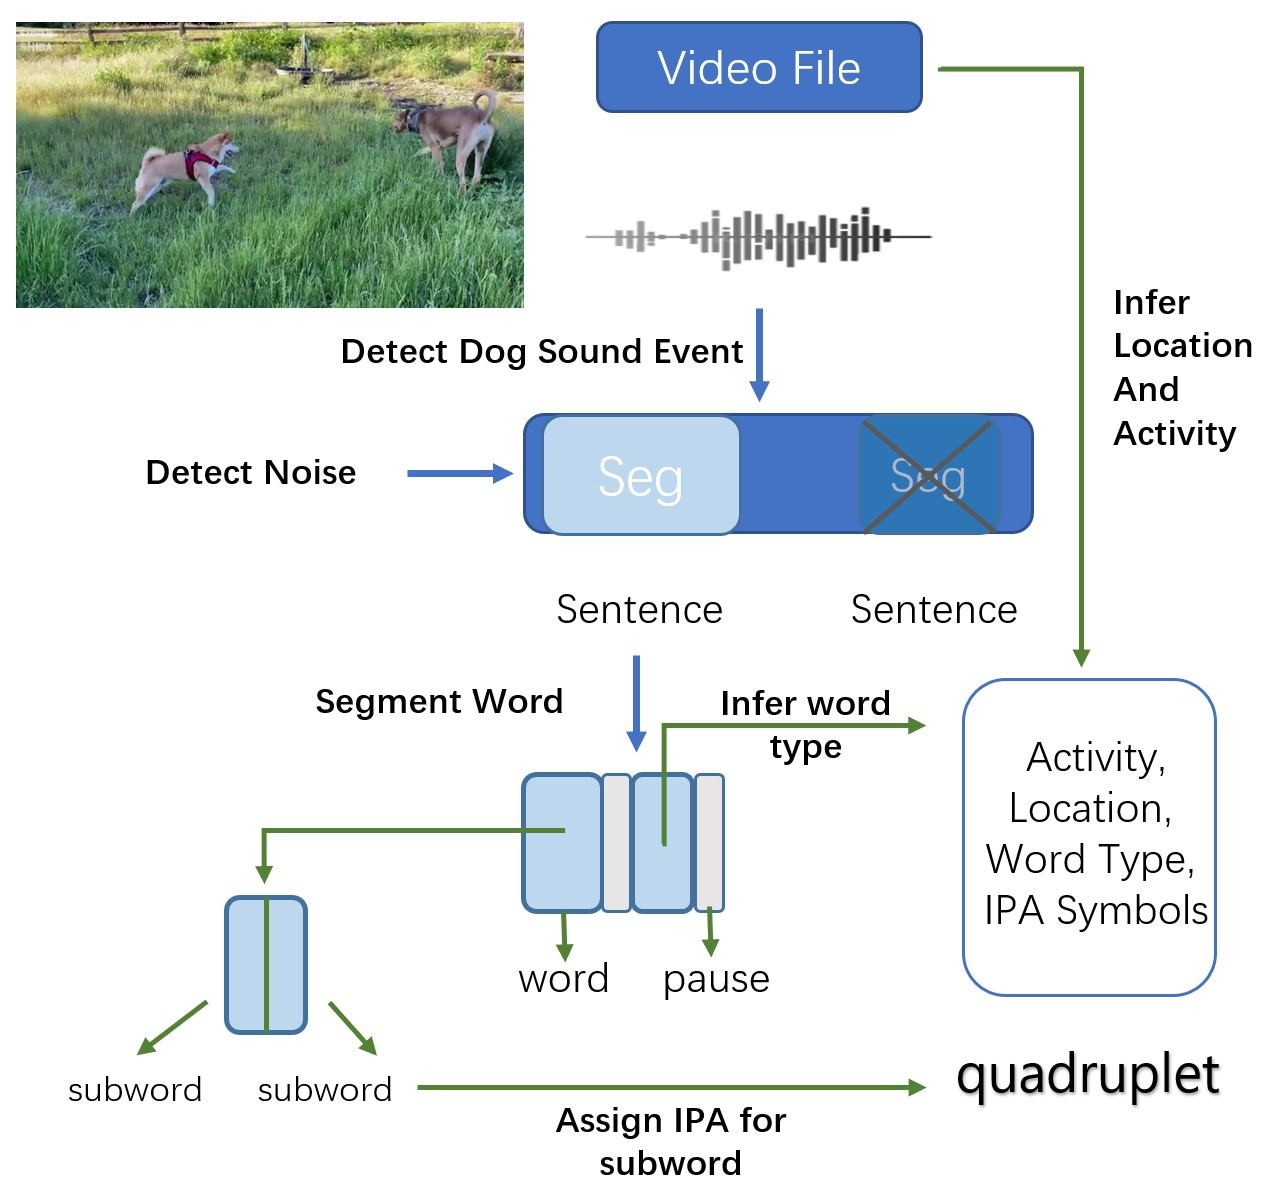
\includegraphics[width=0.9\columnwidth]{images/pipeline.jpg}
	\caption{The overall view of pipeline.}
%\KZ{Word type and subwords should
%be labeled on the two green arrows as well.}}
%Also move "triple" to underneath the figure, so that the fig can fit the whole
%column of the paper. Remove any white space around the pic.}
%\AT{the acc for location and activity will be added by chunhao later}
%\CH{Added}}

%\KZ{Since the dog is the to the left of the bowl in the pic, maybe
%swap the position of the ``food nearby'' and ``begging for food''?}
%Make the pic bigger. Change audio processing to ``word segmentation''.
%No point giving the id of the word, just point out those green segments
%are words. Instead of repeating ``classification model'', say location
%classification and activity classification and the arrows point ``food''
%and ``begging for food'', etc.}
\label{fig:method}
\end{figure}

\subsection{Collect Shiba Inu Online Videos}
\label{sec:collect_data}
% Previous researchers endeavor to uncover the potential patterns in dog language. However, they have often encountered limitations in terms of data availability as they usually record data by themselves in the field or lab. In this work, we collect data from 
%YouTube, which is the largest video portal with millions of videos of dogs. Shiba Inu is widely adopted and has plenty of videos on YouTube and we limit to this breed to avoid differences in semantics between breeds.
%This step enables us to collect mountains of dog videos.
We first use the keyword ``Shiba Inu'' to identify users who own such dogs and only upload shiba inu videos with dog sounds then we collect up to 13,164 Shiba Inu related videos posted by these users within days which can be easily expanded in the future.

\subsection{Sentence Split, Word Segmentation and Subword Extraction}
\label{sec:divide}
Once videos are downloaded, we begin to process the audio tracks.  Similar to human language, where words serve as the fundamental units for constructing sentences, we hypothesize that a similar concept can be applied to dog language. We define a \textbf{``word''} as an independent and contiguous dog vocal sound that typically lasts around 1 second, and it is bounded by some noticeable pauses. A \textbf{``sentence''} is a sequence of consecutive words. A \textbf{``subword''} is a subpart of ``word'' and is represented by an IPA symbol.


%\KZ{The following very important definition can be included in definition
%environment and make them stand out! What's the definition of sub-word?
%You mentioned that too in later parts.}

\paragraph{Sentence Extraction}
%\MY{The below paragraph can be tidying up a bit as well, you define your sentence, and show the purpose of extracting sentence, then say how you did it}

\begin{algorithm}[]
  \SetAlgoLined
  \KwData{Audio tracks}
  \KwResult{``sentences'' of dogs }
  \While{pass accross segments of audio track}
  {
    feed the audio segment feature into PANNs\;
    \eIf{PANNs infers as dog sound without accompanying noise}
    {
      	audio segment belongs to a ``sentence''\;
    }
	{
      pass to next segment\;
  }
  }
  \caption{Sentence Extraction}
%\KZ{Bad english in some of the above 
%statements.}}
\end{algorithm}

To extract the word clips, we adopt a similar methodology as \citet{jieyiacl2023}. The initial step is detecting dog vocalizations and splitting the audio tracks into ``sentences'', continuous sequences of dog vocal sounds. We pass through the frames of audio and determine whether they contain dog sounds. If so, we extract these audio clips and then we remove noise other than dog vocalizations to ensure that there is no accompanying music or human speech in the background. We apply PANNs~\cite{kong2020panns}, a sound event detection model that is pre-trained on the large-scale Audioset~\cite{gemmeke2017audio} dataset with 527 sound classes. 
%\MY{removing sounds other than dog vocalizations and ensure that there's no accompanying music or speech in the background}. 
%This can be detected because they are preceded or followed by 
%significant periods of silence. 
%\KZ{How long is the pause? 
%What's the threshold? It seems that a step is missing, which is first split
%the wave file into sentences by the pauses, and then classify whether each 
%sentence is really a dog sentence, since u can have human sentences or
%music sentences in the output of the first step.}
%\AT{the model predicts whether dog vocalisation and splitting audio according to this result, as explained below}



%To identify a dog ``sentences'', we predict whether the probability of event class 
%``dog'' sound, ${P (\text{dog event}| \text{audio})}$ ranks in the top 10 among all sound classes.
%Then we remove the noisy sentences to ensure the audio clips we got are clean. 
%Due to the nature of YouTube videos, dog sounds are often overlapped with 
%background human speech and music. We excluded those sentences  accompanied by sounds other than ``dog'' and only retained clean ones.  
 %Among the ``sentences'' we got, we remove those from which events ``speech'' or ``music'' are detected in the top 10 events by the PANNS model.


\paragraph{Word Segmentation}
\begin{algorithm}[]
  \SetAlgoLined
  \KwData{``Sentences''}
  \KwResult{``Words''}

  \While{pass through segments of ``sentences''}
  {
    Feed segment feature into PANNs\;
    \eIf{PANNs infers as ``dog'' other than ``silence'' }
    {
      segment belongs to a ``word''\;
    }
	{
      Use segment to split ``words''\;
  }
  }
  \caption{Word Segmentation}
\end{algorithm}


These ``sentences'' may contain short pauses in the middle that can be used to separate the words and the next step is to segment ``words'' in ``sentences''. We finetune PANNs to determine each start and end of a single ``word'' by detecting a frame in the audio clip which transits from a silence frame to a dog frame with a gap of 0.1 seconds between frames. We manually create labels for the event ``dog'' with a total data length of 715 seconds. This finetuned model is capable of detecting the small pauses within ``sentences'' and extracting the singular ``words''. Lastly, we follow the definition of 6 different dog vocalization patterns defined in Audioset, which are distinct from each other. We labeled 240 audio clips and trained a classification model.  
%
% We denote the following variables:
%$T_{\text{dog}}$ as the threshold for the dog voice probability, 
%$T_{\text{silence}}$ as the threshold for the silence probability, 
%$P_{\text{dog}}(t)$ as the probability of the dog voice at time frame $t$, 
%$P_{\text{silence}}(t)$ as the probability of silence at time frame $t$. 
%For an input ``sentence'',  we will decide the start of a dog frame 
%$t_{dog}$ as :
%\begin{align*}
%t_{dog} = \min (t\mid & P_{\text{d}}(t)\ge T_{\text{d}} \text{ and } P_{\text{s}}(t) \le T_{\text{s}} )
%\end{align*}
%where ``d'' refers to dog word and ``s'' refers to silence. 
%We find a frame for the ending of a dog word with the same idea. 

%:
%\begin{align*}
%\text{Change Frame} = \min ( t \mid & P_{\text{dog}}(t) > T_{\text{dog}} \\
%& \text{and } P_{\text{silence}}(t) \leq T_{\text{silence}} )
%\end{align*}
%\MY{rerwite the next few sentences. here you don't want to mention PANNS, say that we follow the definition of 6 different dog vocalization patterns, whcih are distinctive to each other. we labelled xx data and trained a classification model with xx accuracy on the held-out test set. By the end of this step, we obtained a total of xxx different words spreading }

%finetune PANNs as an sound classification model to 
%assign sound type to words % \KZ{shall we use word type here? sound types}:
%The ``words'' we got are sounds from ``sentences'' that sound event ``dog'' is contained. 
%We use the %\KZ{\textit{six dog sound types}} 
%six dog sound types defined in Audioset as all 
%the domains of possible word types in this paper. 
%\KZ{This should go into evaluations:  We also do manual checks and ensure the classification results.} 
%\AT{But we have to finish constructing the triplets so it better be here? I will add a manual check at that part}
 

\begin{equation}
\text{Wordtype} = \arg\max_{i} P_{PANNs}(\text{soundtype}_i | \text{word}).
\end{equation}

%At the end of this process, we have been able to extract small units of 
%dog vocalizations and their corresponding sound type, 
%paving the way for a deeper understanding of their semantic meaning. 

\paragraph{Subword Segmentation and Phonetic Transcription}
We first split ``words'' into ``subwords'' with the method as ~\cite{rasanen2018pre}, which uses sonority fluctuation in audio to segment words into smaller units. Thus, a word can be further split into smaller parts according to the sonority changes. In order to present the vocal characteristics of each subpart, we phonetically transcribe each subword with international phonetic alphabet (IPA) symbols. We compute the acoustic feature distances with standard pronunciations ~\cite{ipa0, ipa1}. In this way, each subword is represented by an IPA vowel symbol, and a ``word'' is represented by a sequence of IPA symbols. 
%we subsequently assign ipa vowel symbols to each subword by calculating euclidien similarity between sound features of subwords and ipa vowels with feature extractor of ~\cite{radford2023robust}\MY{IPA is a term that needs full spell, say that you phonetically transcribe each word with IPA (international phonetic alphabet) symbols.}.
%We average multiple sound tracks to extract the ipa vowel features\MY{this is not complete, you compute the acoustic feature distances with standard pronunciations(quote the original webpage we get these standard sounds), leave out the voice conversion part}, %we also use voice conversion ~\cite{vanniekerk2023rhythm} to augment our ipa vowel sound data. 

\subsection{Surrounding Context Extraction}
\label{sec:infer_context}
% \KZ{Very verbose!}
%After word segmentation, the next task is to find the corresponding contextual information. So far, we have not taken advantage of the visual information in videos. 
Since images and sound are naturally aligned in a video,  we can extract the \textit{location} and \textit{activity} of the dog while it utters a particular ``word'', from the image frames that synchronize with the audio frames. The end product of this phase will be a sequence of quadruplets  consisting of \texttt{<word, subwords, location, activity>}, extracted from the videos. 
% \KZ{set or sequence}

 \paragraph{Location} %\KZ{This para is too long.} 
%In this work, we applied common used methods to acquire these visual 
%information. As for discovering location information, 
%\KZ{is it the begin and end timestamp?}
Given the begin and end timestamp of a ``word'', five image frames in that time range are sampled, then sent into an image classification model to determine the location of the dog when the ``word'' occurs. Here we finetune the pre-trained model from~\citet{zhou2017places} trained on the scene-centric datasets Places365 based on thousands of pictures sampled from Shiba Inu videos to predict the dog's location. The fine-tuned model achieves 77.99\% on Top-1 accuracy and 97.13\% on Top-5 accuracy. 
%\KZ{What model?
%how was this model trained?} 
 
We denote the following variables:
$t_{\text{word}}$: Timestamp of the ``word'' occurrence between begin and end, %\KZ{Begin or end?}
$I_{\text{i}}$: An image from a batch of images constructed from five frames sampled around the timestamp $t_{\text{word}}$,
$M_{\text{class}}$: The class predicted by the model given $I_{\text{i}}$,
$L_{\text{dog}}$: Location of the dog when the ``word'' occurs,
$\text{Majority Vote}$ is a function that selects the class with the highest frequency among the predicted class of the individual images in the batch.
The formula for location inference is as:
\begin{equation}
L_{\text{dog}} = \text{Majority Vote}\left(\bigcup_{i=1}^{n} M_{\text{class}}(I_i)\right)
\end{equation}

%\begin{equation}
%L_{\text{dog}} = M_{\text{classification}}(I_{\text{batch}})
%\end{equation}
%\KZ{This equation is not right: a classifier only takes 1 image as input.
%How do you handle 5? Is it majority voting, or what?}


%Since we mainly want to extract location information about the background rather than the subject, we choose the pre-trained model from~\cite{zhou2017places} which is trained on the scene-centric datasets Places365 and finetuned it based on 2000 human annotated pictures sampled from Shiba Inu videos. 
%As for discovering location information, given the timestamp of a ``word'', five frames from the video are sampled out, constructed into a batch of images that could reflect the location information, and the batch is then sent into an image classification model to judge what's the location of the dog when the ``word'' occurs. Since we mainly want to extract location information about the background rather than the subject, we choose the pre-trained model from~\cite{zhou2017places} which is trained on the scene-centric datasets Places365 and finetuned it based on thousands of pictures sampled from Shiba Inu videos. 
%As for discovering location information, given the timestamp of a ``word'', five frames from the video are sampled out, constructed into a batch of images which could reflect the location information, and the batch is then sent into an image classfication model to judge what's the location of the dog when the ``word'' occurs. Since we mainly want to extract location information about the background rather than the subject, we choose the pretrained model from~\cite{zhou2017places} which is trained on the scene-centric datasets Places365 and finetuned it based on thousands of pictures sampled from Shiba Inu videos. \KZ{This should be
%in the eval section: }

%The finetuned model achieves an accuracy of 77.99\% on our manually labeled pictures.

%To get the activity information about the dog, we sample a five-second video clip based on the timestamp of the ``word'', and then a video understanding model is applied to decide what the dog is doing. The pre-trained model TSN~\cite{wang2018temporal} performs well on the task of video understanding. In this study, we annotated a set of video clips sampled from the Shiba Inu videos and finetuned the pre-trained model. Based on the finetuned models, given the timestamp of a ``word'', we can explore the location and activity from the video. 
%To get the activity information about the dog, we sample a five-second video clip based on the timestamp of the ``word'', and then a video understanding model is applied to decide what the dog is doing. The pretrained model TSN~\cite{wang2018temporal} performs well on the task of video understanding. In this study, we annotated a set of video clips sampled from the Shiba Inu videos and finetuned the pre-trained model. The finetuned model achieves an top1 accuracy of 59.11\% and top5 accuracy of 94.16\%. Based on the finetuned models, given the timestamp of a ``word'', we can explore the location and activity from the video. 


\paragraph{Activity} To get the activity information about the dog, we sample a five-second video clip based on the timestamp of the ``word'' that we chooce a range of (begin timestamp  - 1s, end timestamp + 1s), and then a video understanding model is applied to decide what the dog is doing. The pre-trained model Temporal Segment Networks~(TSN)~\cite{wang2018temporal} performs well on the task of video understanding. In this study, we annotated 2534 video clips sampled from the Shiba Inu videos and finetune the pre-trained model. The fine-tuned model achieves 61.40\% on Top-1 accuracy and 92.40\% on Top-5 accuracy. Based on these two fine-tuned models, given the timestamp of a ``word'', we can explore the location and activity from the video.
% \MY{spell TSN in full first}
%$Activity_{dog} = Model(I_{t})$
%where $I_{t}$ refers to a batch of audio clips constructed around the timestamp %$t_{\text{word}}$.
%\KZ{this and the previous formula are useless.}

%\subsection{Implementation Details}
%We use PANNs ~\cite{kong2020panns} to extract ``sentences''. For removing noises, if PANNs infers there is human voice or background music, we will remove these clips. For extracting ``words'', we finetune PANNs on our humain annotated short dog word dataset. For classifing the type of the word, we select the word type predicted by PANNs with highest probability. We also do manual check and ensure the classification results. 
